In this chapter we introduce the mathematical models for the object tracking problem which will be used throughout the rest of this report.

We first assume that our targets exist at singular points in space, and that targets move independently of each other. Each target will be characterised by a state vector $x_{j,t}$. This state is composed of continuous-valued coordinates and evolves according to a hidden Markov model (HMM)

\begin{equation}
x_{j,t} \sim P(x_{j,t}|x_{j,t-1}).
\end{equation}

At first, we will also assume that we know how many targets are in the scene and their starting locations, $\{x_{j,0}\}$.

The targets are observed by a sensor which detects each with a probability $P_D$. If detected, the sensor returns a point observation at a location $y_t^{(i)}$ given by

\begin{equation}
y_t^{(i)} \sim P(y_t|x_{j,t}).
\end{equation}

In addition to the observations originating from targets, the sensor also detects a number of false alarms. We assume that these are generated by a Poisson process, with a uniform intensity over the observation area. The expected number of clutter observations in a frame is denoted $\mu_C$.

We denote the set of targets present as $X_t = \{x_{1,t}, x_{2,t}, ... , x_{K_t, t} \}$, and the set of observations as $Y_t = \{y_t^{(1)}, y_t^{(2)}, ... , y_t^{(M_t)} \}$.

We introduce an association variable for each target, $\lambda_{j,t}$, which indicates which of the observations in that frame was generated by this target, as shown in figure~\ref{fig:BasicTrackingAssoc}. If the target is not detected, then $\lambda_{j,t}$ is set to 0. We denote the set $\Lambda_t = \{\lambda_{1,t}, \lambda_{2,t}, ... , \lambda_{K_t, t} \}$. As each observation is generated by one target or clutter, no two elements of $\Lambda_t$ may take the same value, unless 0. (This is the constraint that the PMHT and PDAF relax.)

\begin{figure} \centering
\input{BasicTrackingAssoc.pdf_tex}%
\caption{A simple two-target tracking problem illustrating the different possible associations at one time step. Hidden states shown as blue crosses. Observations shown as red circles.}
\label{fig:BasicTrackingAssoc}%
\end{figure}

The graphical model including the association variables is shown in figure~\ref{fig:HMMAssoc}.

\begin{figure}%
\centering

\tikzstyle{state} = [circle,thick,minimum size=1.2cm,draw=black]
\tikzstyle{assoc} = [circle,thick,minimum size=1.2cm,draw=blue]
\tikzstyle{observ} = [circle,thick,minimum size=1.2cm,draw=red]

\begin{tikzpicture}[>=latex,text height=1.5ex,text depth=0.25ex]

	\matrix[row sep=0.5cm,column sep=0.5cm] {
		&
		\node (y_k-1) [observ]{$Y_{k-1}$}; &
		&
		\node (y_k) [observ]{$Y_{k}$}; &
		&
		\node (y_k+1) [observ]{$Y_{k+1}$}; &
		& \\
		& &
		\node (l_k-1) [assoc]{$\Lambda_{k-1}$}; &
		&
		\node (l_k) [assoc]{$\Lambda_{k}$}; &
		&
		\node (l_k+1) [assoc]{$\Lambda_{k+1}$}; & \\
		\node (x_k-2) {$\cdots$}; &
		\node (x_k-1) [state]{$X_{k-1}$}; &
		&
		\node (x_k) [state]{$X_{k}$}; &
		&
		\node (x_k+1) [state]{$X_{k+1}$}; &
		&
		\node (x_k+2) {$\cdots$}; \\
	};

	\path[->]
		(x_k-2) edge[thick] (x_k-1)
		(x_k-1) edge[thick] (x_k)
		(x_k) edge[thick] (x_k+1)
		(x_k+1) edge[thick] (x_k+2)
		
		(x_k-1) edge[thick] (y_k-1)
		(x_k) edge[thick] (y_k)
		(x_k+1) edge[thick] (y_k+1)
		
		(l_k-1) edge[thick] (y_k-1)
		(l_k) edge[thick] (y_k)
		(l_k+1) edge[thick] (y_k+1)
		;

\end{tikzpicture}
\caption{Graphical model for tracking including association variables.}%
\label{fig:HMMAssoc}%
\end{figure}

If we wished to calculate the posterior distribution over the target states, $X_t$, we would need to marginalise the association variables in the calculation of the likelihood term

\begin{equation}
P(Y_t|X_t) = \sum_{\Lambda_t} P(Y_t|X_t, \Lambda_t) P(\Lambda_t)
\label{eq:MarginaliseAssociations}
\end{equation}

where the summation is over all feasible values of $\Lambda_t$. The number of terms in this summation combinatorially in the number of targets and the number of observations, and may be prohibitively large if there are many targets or observations in the scene. If it is necessary to calculate the likelihood very often, as in a particle filter, it may be preferable to estimate $\Lambda_t$ instead of marginalising it. The target distribution is now

\begin{equation}
P(X_{1:t}, \Lambda_{1:t}|Y_{1:t}) = \frac{P(Y_t|X_t, \Lambda_t) P(X_t|X_{t-1}) P(\Lambda_t) P(X_{1:t-1}, \Lambda_{1:t-1}|Y_{1:t-1})}{P(Y_t|Y_{1:t-1})}.
\label{eq:MTPosterior}
\end{equation}

We now consider the terms of this equation one at a time.

\section{Observation likelihood}
The likelihood given the associations is given by

\begin{equation}
P(Y_t|X_t, \Lambda_t) = V^{-(M_t-M_{T,t})} \prod_{\lambda_{j,t} \ne 0} P(y_t^{(\lambda_{j,t})}|x_{j,t})
\label{eq:MTLikelihood}
\end{equation}

where $V$ is the volume of the observation region, and thus $V^{-1}$ is the likelihood of a clutter observation, and where $M_{T,t} = \left| \{ \lambda_{j,t} \ne 0 \} \right|$. This can be conveniently factorised as

\begin{equation}
P(Y_t|X_t, \Lambda_t) = V^{-(M_t-K_t)} \prod_{j=1}^{K_t} \begin{cases} P(y_t^{(\lambda_{j,t})}|x_{j,t}) & \lambda_{j,t} \ne 0 \\ V^{-1} & \lambda_{j,t} = 0 \end{cases}.
\label{eq:MTFactorisedLikelihood}
\end{equation}

This expression contains a factor for each target, and a coefficient independent of the state. This coefficient will either cancel out (MCMC) or be discarded in the weight normalisation (SISR), and can thus be neglected.



\section{Transition dynamics}
Similarly, because of our independence assumption on the targets, the transition dynamic term will factorise as a product of target-specific terms

\begin{equation}
P(X_t|X_{t-1}) = \prod_{j=1}^{K_t} P(x_{j,t}|x_{j-1}).
\label{eq:MTFactorisedTransition}
\end{equation}



\section{Association likelihood}
The association variable, $\Lambda_t$, tells us how many targets have been detected (and how many have not), and how many clutter observations are present. To construct a prior distribution on this, consider the $\lambda_{j,t}$s in turn. Each one can be either 0 with probability $(1-P_D)$, or an observation index with probability $P_D$. If it is the latter, there are $M_t - M_{\textnormal{taken}}$ indexes from which to choose, where $M_{\textnormal{taken}}$ is the number of observations already assigned to a previous target. Once we have considered all the targets, $M_{T,t}$ observations will have been assigned to targets, and all those remaining must be generated by the clutter process. The number of these is Poisson distributed. The association prior for feasible is $\Lambda_t$ thus given by

\begin{IEEEeqnarray}{rCl}
P(\Lambda_t) & = & \underbrace{\frac{P_D^{M_t}}{M_t(M_t-1)...(M_t-M_{T,t})}}_\textnormal{detected targets} \underbrace{(1-P_D)^{(K-M_t)}}_\textnormal{undetected targets} \underbrace{\frac{\exp(-\mu_C) \mu_C^{(M_t-M_{T,t})}}{(M_t-M_{T,t})!}}_\textnormal{clutter} \nonumber \\
 & = & \frac{ \exp(-\mu_C) \mu_C^{(M_t-M_{T,t})} P_D^{M_t} (1-P_D)^{(1-M_t)} }{ M_t! }
\label{eq:MTAssociationLikelihood}
\end{IEEEeqnarray}

while for invalid $\Lambda_t$ ($\lambda_{i,t}=\lambda_{j,t}$ for $i \ne j$, $\lambda_{i,t},\lambda_{j,t} \ne 0$), the probability is zero. Again, we can factorise this expression over the targets

\begin{equation}
P(\lambda_t) = \frac{\exp(-\mu_C) \mu_C^{(M_t-K_t)}}{M_t!} \prod_{j=1}^{K_t} \begin{cases} P_D & \lambda_{j,t} \ne 0, \lambda_{j,t} \notin \{ \lambda_{1:j-1,t} \} \\ 0 & \lambda_{j,t} \in \{ \lambda_{1:j-1,t} \} \\ (1-P_D) \mu_C & \lambda_{j,t}=0 \end{cases}.
\label{eq:MTFactorisedAssociationLikelihood}
\end{equation}

Just as for the observation likelihood, this expression has a factor for each target and a state-independent coefficient which can be neglected for either a SISR or MCMC particle filter.



\section{Assumptions}
Here we summarise the assumptions made in the model formulations:

\begin{itemize}
	\item Targets and observations occur at singular points.
	\item The number of targets is known.
	\item Target starting locations known.
	\item Target states evolve independently of each other according to a HMM.
	\item Targets are detected in each frame with an independent probability $P_D$. A detected target generates one observation.
	\item A single target is associated with each observation.
	\item Clutter observations are generated by a homogeneous spatial Poisson process.
\end{itemize}



\section{Specific models}

\subsection{State transitions}
Throughout this work we employ a Near-Constant Velocity (NCV) model. We omit the target index $j$ in the following and consider only a single spatial dimension. The extension to multiple dimensions is trivial. A target state, $x$, is written as a vector

\begin{equation}
x = \begin{pmatrix}
	s \\ \dot{s}
\end{pmatrix}.
\end{equation}

We define the target motion by a simple stochastic differential equation, in which acceleration is a Wiener process

\begin{IEEEeqnarray}{rCl}
d\dot{s}_{\tau} & = & \sigma dW_{\tau} \\
ds_{\tau} & = & \dot{s}_{\tau}.
\end{IEEEeqnarray}

Integrating these gives us

\begin{IEEEeqnarray}{rCl}
\dot{s}_{\tau} & = \dot{s}_0& + \sigma W_{\tau} \\
s_{\tau} & = & s_0 + \dot{s}_0 {\tau} + \sigma \int_0^{\tau} W_s ds
\end{IEEEeqnarray}

which we can rewrite in matrix form

\begin{equation}
\begin{bmatrix}s_{\tau} \\ \dot{s}_{\tau}\end{bmatrix} = \begin{bmatrix}1 & {\tau} \\ 0 & 1\end{bmatrix} \begin{bmatrix}s_0 \\ \dot{s}_0\end{bmatrix} + \sigma \begin{bmatrix}W_{\tau} \\ \int_0^{\tau} W_s ds \end{bmatrix}.
\end{equation}

It is thus clear that the $x_{\tau}|x_0$ is normally distributed with mean $x_0$ and covariance 

\begin{equation}
\mathbb{V}[x_{\tau}] = \sigma^2 \mathbb{E}\begin{bmatrix}W_{\tau}^2 & W_{\tau} \int_0^{\tau} W_s ds \\ W_{\tau} \int_0^{\tau} W_s ds & \left( \int_0^{\tau} W_s ds \right)^2\end{bmatrix} = \sigma^2 \begin{bmatrix} {\tau} & \frac{{\tau}^2}{2} \\ \frac{{\tau}^2}{2} & \frac{{\tau}^3}{3}\end{bmatrix}.
\end{equation}

The model can now be discretised onto a set of time points, indexed with $t$. The transition density is linear-Gaussian given by

\begin{equation}
P(x_{t+1}|x_{t}) = \mathcal{N}(x_{t+1}|A x_{t},Q).
\end{equation}

Throughout this report, we will consider models in two spatial dimensions. Thus the matrices $A$ and $Q$ are given by

\begin{equation}
A = \begin{bmatrix}
1 & 0 & P & 0 \\
0 & 1 & 0 & P \\
0 & 0 & 1 & 0 \\
0 & 0 & 0 & 1
\end{bmatrix}
\end{equation}

\begin{equation}
Q = \sigma^2 \begin{bmatrix}
P & 0 & \frac{P^2}{2} & 0 \\
0 & P & 0 & \frac{P^2}{2} \\
\frac{P^2}{2} & 0 & \frac{P^3}{3} & 0 \\
0 & \frac{P^2}{2} & 0 & \frac{P^3}{3} \\
\end{bmatrix}
\end{equation}

and where $P$ is the sampling period.



\subsection{Observations}
We will use two different observation models. Firstly, linear-Gaussian where the position is observed directly

\begin{equation}
P(y_t^{\lambda_t}|x_t) = \mathcal{N}(y_t^{\lambda_t}|C x_t, R)
\end{equation}

where $C$ is

\begin{equation}
\begin{bmatrix}
1 & 0 & 0 & 0 \\
0 & 1 & 0 & 0 \\
\end{bmatrix}.
\end{equation}

Secondly, we consider a polar observation model, of the form used for radar systems

\begin{equation}
P(y_t^{\lambda_t}|x_t) = \mathcal{N}(y_t^{\lambda_t}|h(x_t), R)
\end{equation}

where

\begin{equation}
h(x_t) = \begin{bmatrix}
\arctan \left( \frac{x_{2,t}}{x_{1,t}} \right)\\
\sqrt{ (x_{1,t}^2 + (x_{2,t}^2 }
\end{bmatrix}.
\end{equation}

We will need a linearised, EKF approximation of this model for use in proposal distributions. This will require the Jacobian of the observation function

\begin{equation}
C_t = \begin{bmatrix} \frac{\partial h_1}{\partial x_{1,t}} & \frac{\partial h_1}{\partial x_{2,t}} & \frac{\partial h_1}{\partial \dot{x}_{1,t}} & \frac{\partial h_1}{\partial \dot{x}_{2,t}} \\ \frac{\partial h_2}{\partial x_{1,t}} & \frac{\partial h_2}{\partial x_{2,t}} & \frac{\partial h_2}{\partial \dot{x}_{1,t}} & \frac{\partial h_2}{\partial \dot{x}_{2,t}} \end{bmatrix}
= \begin{bmatrix} \frac{-x_{2,t}}{x_{1,t}^2 + x_{2,t}^2} & \frac{x_{1,t}}{x_{1,t}^2 + x_{2,t}^2} & 0 & 0 \\ \frac{x_{1,t}}{\sqrt{x_{1,t}^2 + x_{2,t}^2}} & \frac{x_{2,t}}{\sqrt{x_{1,t}^2 + x_{2,t}^2}} & 0 & 0 \end{bmatrix}.
\end{equation}

The effect of such an approximation is illustrated in figure~\ref{fig:EKFradar}

\begin{figure}[!hbt] \centering
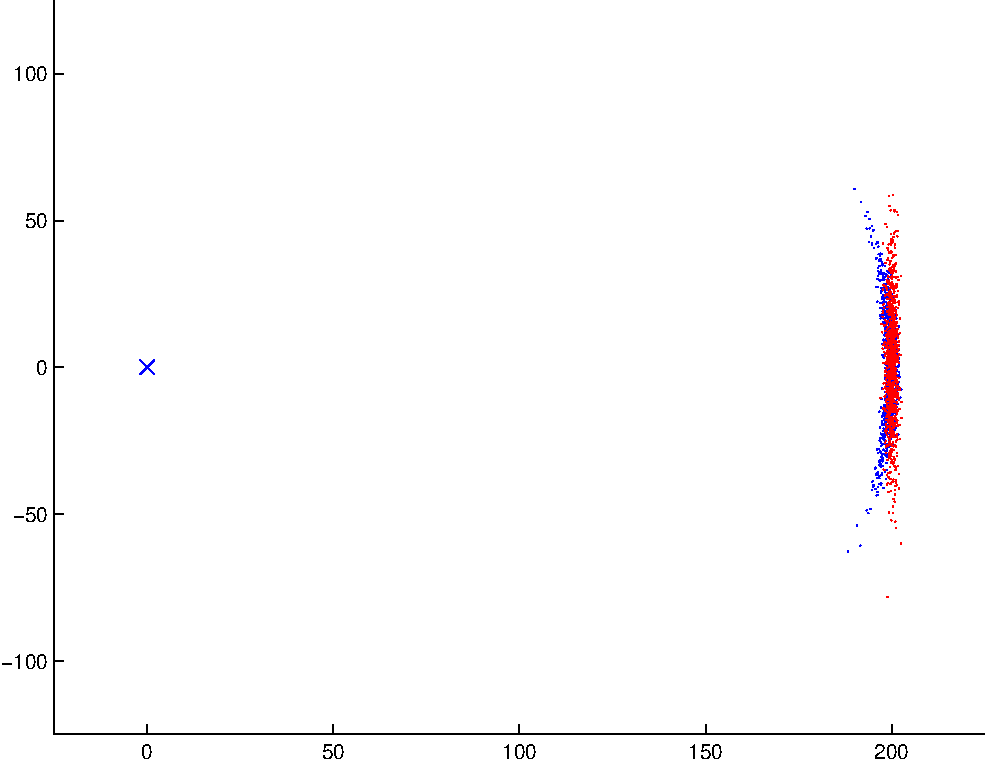
\includegraphics[width=0.7\columnwidth]{EKF-crop.pdf}%
\caption{Samples from the nonlinear observation distribution (blue) and from the EKF approximation (red).}%
\label{fig:EKFradar}%
\end{figure}
